%----------------------- Wydruk dwustronny ---------------
%\documentclass[12pt,twoside,a4paper]{book} % 
%----------------------- Wydruk jednostronny ---------------
%\documentclass[draft,12pt,oneside,a4paper]{book} % jednostronnego
%opcja draft pozwala na szybką kompilację bez obrazków
\documentclass[12pt,oneside,a4paper]{book} % jednostronnego
%#################### packages############################
\usepackage[QX]{polski}
\usepackage[utf8]{inputenc}
%\usepackage{latexsym}
%\usepackage{tgpagella}
\usepackage{lmodern}
\usepackage{amsmath,amsthm,amsfonts,amssymb,alltt}
%\usepackage{epsfig}
%\usepackage{pdflscape}
%\usepackage{caption}
%\usepackage{indentfirst}
%\usepackage{cite}
%\usepackage{boondox-calo}

\usepackage{float}
\usepackage{graphicx}
\usepackage{subcaption}

\usepackage{color}
\usepackage[x11names,dvipsnames,table]{xcolor}
\usepackage{hyperref}
\hypersetup{
pdfauthor={Imie Nazwisko},
colorlinks=True,
linkcolor=darkgray,  % color of internal links (change box color with linkbordercolor)
citecolor=BrickRed,  % color of links to bibliography
filecolor=Magenta,   % color of file links
urlcolor=BlueViolet}	%%pdfpagemode=FullScreen}

\usepackage[linesnumbered,lined,commentsnumbered, algochapter]{algorithm2e}
\SetKwFor{ForEach}{for each}{do}{end for}%
\SetKwFor{ForAll}{for all}{do}{end for}%
\newenvironment{myalgorithm}
{\rule{\textwidth}{0.5mm}\\\SetAlCapSty{}\SetAlgoNoEnd\SetAlgoNoLine\begin{algorithm}}{\end{algorithm}\rule{\textwidth}{0.5mm}}


%---------------------
\overfullrule=2mm
\pagestyle{plain}
\textwidth=15cm \textheight=685pt \topmargin=-25pt \linespread{1.3} 
\setlength{\parskip}{0pt}
\setlength\arraycolsep{2pt}
\oddsidemargin =0.9cm
\evensidemargin =-0.1cm

%---------------------


\usepackage{color}

\newtheorem{tw}{Twierdzenie}[chapter]
\newtheorem{lem}[tw]{Lemat}
\newtheorem{co}[tw]{Wniosek}
\newtheorem{prop}[tw]{Stwierdzenie}
\theoremstyle{definition}
\newtheorem{ex}{Przykład}
\newtheorem{re}[tw]{Uwaga}
\newtheorem{de}{Definicja}[chapter]



\newcommand{\bC}{{\mathbb C}}
\newcommand{\bR}{{\mathbb R}}
\newcommand{\bZ}{{\mathbb Z}}
\newcommand{\bQ}{{\mathbb Q}}
\newcommand{\bN}{{\mathbb N}}
\newcommand{\captionT}[1]{\caption{\textsc{\footnotesize{#1}}}}
\renewcommand\figurename{Rys.}

\numberwithin{equation}{chapter}
\renewcommand{\thefootnote}{\arabic{footnote})}
\usepackage{fancyhdr}   % w tym dokumencie deklarujemy potrzebne pakiety
%#################### packages############################

%\definecolor{mygreen}{rgb}{0,0.6,0}
\definecolor{mygray}{rgb}{0.92,0.92,0.92}
\definecolor{light-gray}{gray}{0.85}
\definecolor{mymauve}{rgb}{0.58,0,0.82}
%\definecolor{myred}{rgb}{1,0,0}


\usepackage{listings}
% wspólny licznik dla figures and lislistings
\makeatletter
\AtBeginDocument{%
  \let\c@figure\c@lstlisting
  \let\thefigure\thelstlisting
  \let\ftype@lstlisting\ftype@figure % give the floats the same precedence
}
\makeatother
%----------------------------------------
\usepackage{listingsutf8}
\renewcommand{\lstlistingname}{Rys.}%{Kod \'{z}r\'{o}d\l{l}owy}
\lstset{
basicstyle=\ttfamily ,
language=python,
inputencoding=utf8/cp1250,
extendedchars=true,
numbers=left, %eller none
numberstyle=\scriptsize\color{black}\bfseries,
%frame = tb,
captionpos = rb,
backgroundcolor=\color{light-gray},
xleftmargin=\parindent,
% xrightmargin=3.5cm
showstringspaces=false,
commentstyle=\color{Red},
keywordstyle=\color{YellowOrange},
keywordstyle=[2]\color{RedViolet},
keywords={and,del,from,not,while,as,elif,global,or,with,assert,else,if,pass,yield,break,
except,import,class,exec,in,raise,continue,finally,is,return,def,for,lambda,try},
keywords=[2]{print,object,type,input,sum,min,max,int,float,str,list,dict,set,tuple},
rulesepcolor=\color{Blue},
escapeinside={<@}{@>},
stringstyle=\color{OliveGreen},
%basicstyle=\color{Black},
%morecomment=[l]\#,%
morestring=[d]{\\'},
morestring=[d]{\\"},
%morestring=[b]',%
%morestring=[b]",%
%morestring=*[d]',%
%morestring=*[d]",%
%morestring=[d]{\\'},
%morestring=**[d]{"},
%morestring=[d]{\\"},
morestring=[s]{'}{'},
morestring=[s]{"}{"},
morestring=[s]{'''}{'''},
morestring=[s]{"""}{"""},
morestring=[s]{f"""}{"""},
morestring=[s]{r"""}{"""},
morestring=[s]{f"}{"},
morestring=[s]{f'}{'},
morestring=[s]{r"}{"},
morestring=[s]{r'}{'},
morecomment=[s]{Traceback}{Error*},
literate={ą}{{\k{a}}}1
             {Ą}{{\k{A}}}1
             {ę}{{\k{e}}}1
             {Ę}{{\k{E}}}1
             {ó}{{\'o}}1
             {Ó}{{\'O}}1
             {ś}{{\'s}}1
             {Ś}{{\'S}}1
             {ł}{{\l{}}}1
             {Ł}{{\L{}}}1
             {ż}{{\.z}}1
             {Ż}{{\.Z}}1
             {ź}{{\'z}}1
             {Ź}{{\'Z}}1
             {ć}{{\'c}}1
             {Ć}{{\'C}}1
             {ń}{{\'n}}1
             {Ń}{{\'N}}1
}


 % definicja wyglądu kodu żródłowego 


%-----------------właściwa część pracy-----------------

\begin{document}
%jak dokument jest duży dobrym pomysłem jest podział dokumentu na wiele plików %mozna to też zrobić z rozdziałami
% \thispagestyle{empty}


%\begin{center}

{\large
Przedmiot: Wstęp do Imagineskopii\\
TEMAT : Ogólna teoria wszystkiego\\
Imię Nazwisko Grupa : LX
}

%\end{center}




%\thispagestyle{empty} \setcounter{page}{0} \tableofcontents



\chapter{Mroczek Adrian - Zadanie nr. 2 Fourier }

\begin{figure}[h]
\begin{center} 
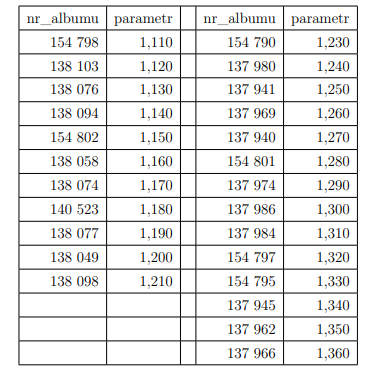
\includegraphics[scale=1]{./images/02.PNG} 
\caption{\textit{Przypis parametru do numeru albumu}.\newline }
%do spisy tresci wersja skrócona
\label{rys:logoup}
\end{center}
\end{figure}



\begin{figure}[h]
\begin{center} 
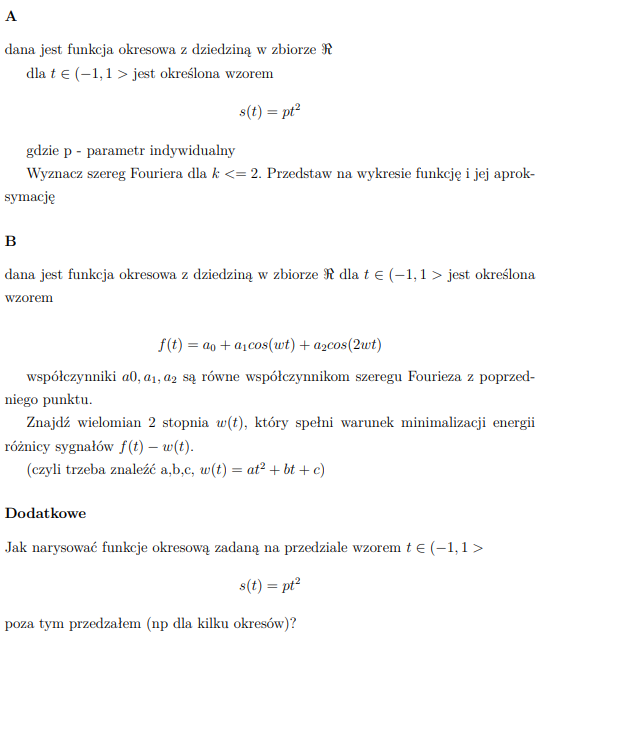
\includegraphics[scale=0.9]{./images/ZadanieSyganly.PNG} 
\caption{\textit{Zadanie Fourier}.\newline }
%do spisy tresci wersja skrócona
\label{rys:logoup}
\end{center}
\end{figure}

\chaptermark{Wzory...}

% Dane do obliczeń:\newline
% C=0.001
% R=1NNN, gdzie NNN to 3 ostatnie cyfry albumu (czyli jak np albumu kończy się na 045 to R=1045).\newline
% Moje Dane do obliczeń:\newline
% Nr albumu = 137980, z tego wynika ze R = 1980.  

% \subsection{Wzór klasyczny}


% fsdf

% \thispagestyle{empty} \addcontentsline{toc}{chapter}{Wstęp}




% % \subsection{Obliczenie alfa}

% \begin{figure}[h]
% \begin{center} 

% 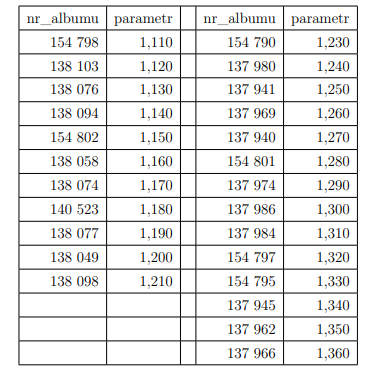
\includegraphics[scale=0.7]{./images/02.PNG}

% \caption{\textit{Wstępne obliczenie alfa}.\newline }
% %do spisy tresci wersja skrócona
% \label{rys:logoup}
% \end{center}
% \end{figure}

% % \subsection{Reszta obliczeń}
% \begin{figure}[h]
% \begin{center} 

% 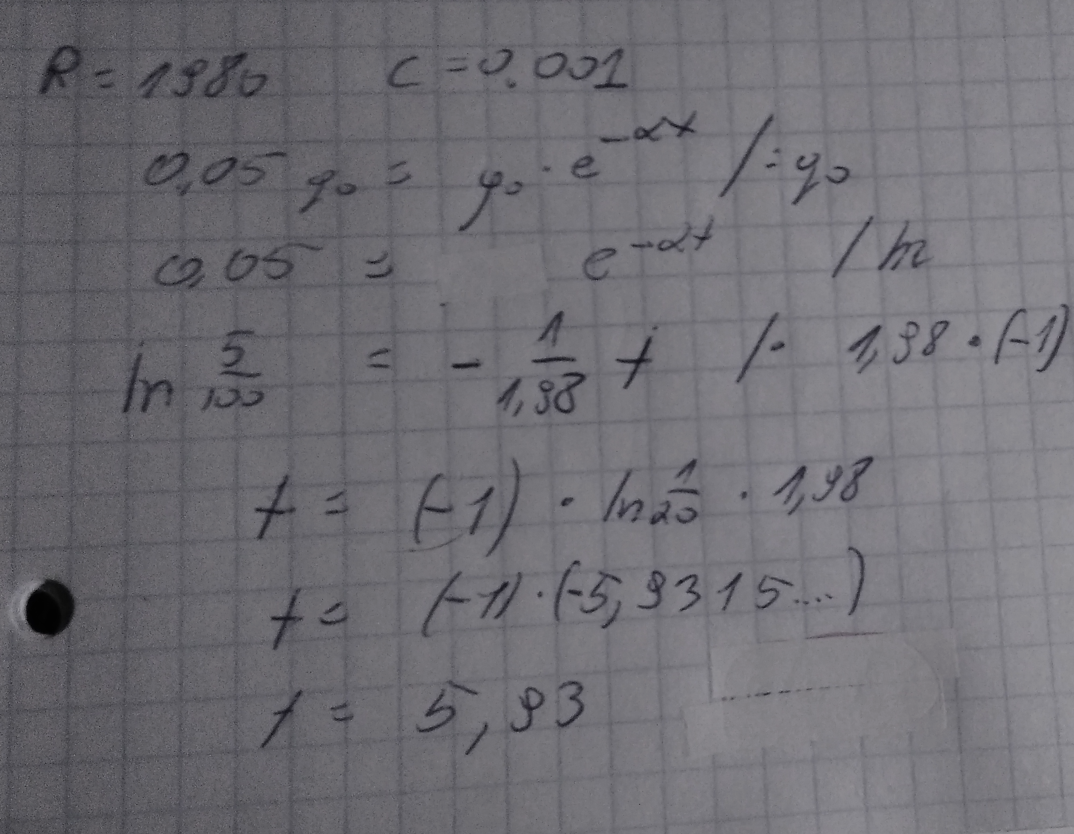
\includegraphics[scale=0.5]{./images/01.PNG} 

% \caption{\textit{Obliczenia}.\newline }
% %do spisy tresci wersja skrócona
% \label{rys:logoup}
% \end{center}
% \end{figure}

% \begin{figure}[h]
% \begin{center} 
% 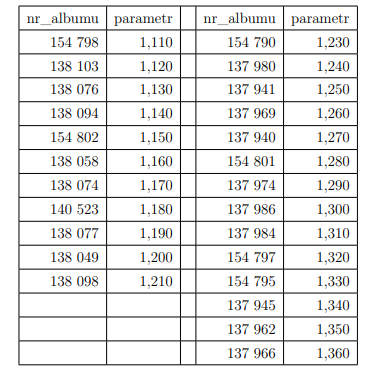
\includegraphics[scale=0.7]{./images/02.PNG}
% \caption{\textit{Wstępne wzory}.\newline }
% %do spisy tresci wersja skrócona
% \label{rys:logoup}
% \end{center}
% \end{figure}


\chapter{Mroczek Adrian - Rozwiazanie A  }
% \section{Dane do zadania}
% Nr albumu = 137 980   p = 1,240


\begin{figure}[h]
\begin{center} 
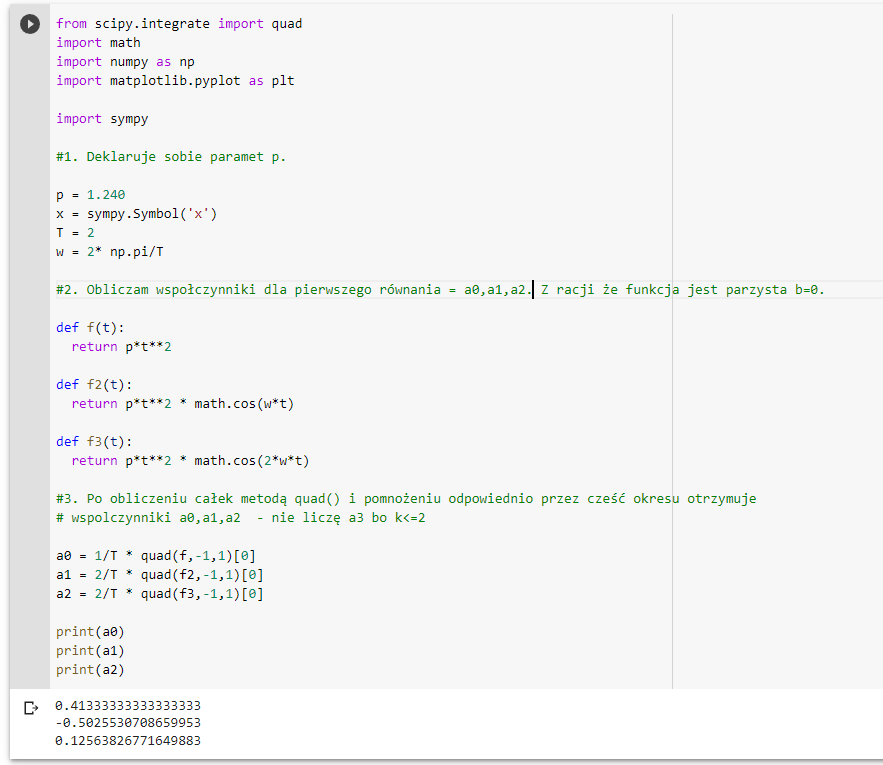
\includegraphics[scale=0.7]{./images/RozwiazanieA.PNG} 
\caption{\textit{Kod w pythonie z komentarzem.}\newline }
%do spisy tresci wersja skrócona
\label{rys:logoup}
\end{center}
\end{figure}


% \section{Rozwiązanie}
% % 2. Przyjąć że po tym czasie odpowiedź swobodna zanikła i badać dalej tylko część
% % odpowiedzi wymuszeniowej. Zbadać zależność amplitudy q(t) oraz i(t) w zależności
% % od częstości wymuszenia w przedziale (0.1,10)..Wykonać wykres A(w). Oś częstości przedstawić w skali logarytmicznej
% % o podstawie 10. Wyznaczenie maksimum funkcji można wykonać przez tablicowanie funkcji z małym krokiem.

% \chaptermark{Wzory...}
% % \section{Niech u(t) = C * sin(wt)}


% \begin{figure}[h]
% \begin{center} 
% 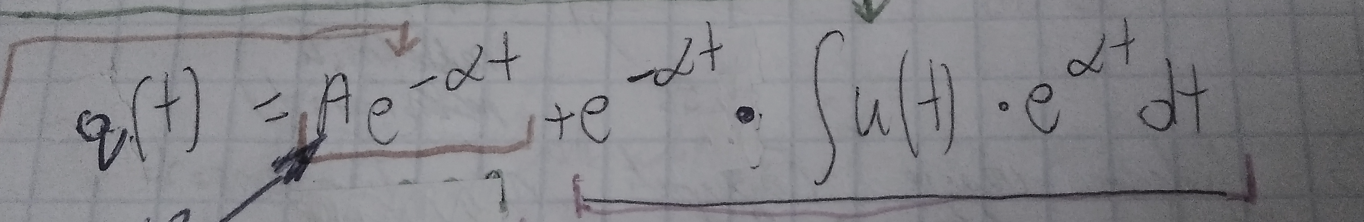
\includegraphics[scale=0.7]{./images/001.PNG} 
% \caption{\textit{Suma drgań własnych (które wygasają po czasie 5.93s) oraz odpowiedzi układu po ustabilizowaniu się}.\newline }
% %do spisy tresci wersja skrócona
% \label{rys:logoup}
% \end{center}
% \end{figure}


% \begin{figure}[h]
% \begin{center} 
% 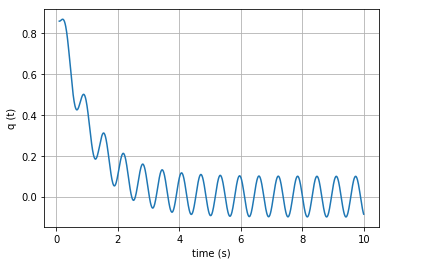
\includegraphics[scale=0.8]{./images/czestosc=10.PNG} 
% \caption{\textit{Badanie dla częstości = 10}.\newline }
% %do spisy tresci wersja skrócona
% \label{rys:logoup}
% \end{center}
% \end{figure}


% \begin{figure}[h]
% \begin{center} 
% 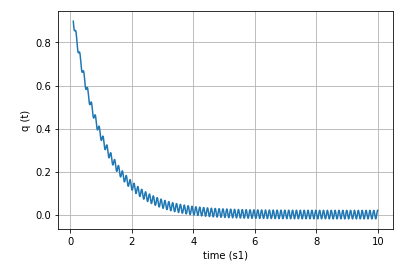
\includegraphics[scale=0.8]{./images/czestosc=50.PNG} 
% \caption{\textit{Badanie dla częstości = 50}.\newline }
% %do spisy tresci wersja skrócona
% \label{rys:logoup}
% \end{center}
% \end{figure}


% \begin{figure}[h]
% \begin{center} 
% 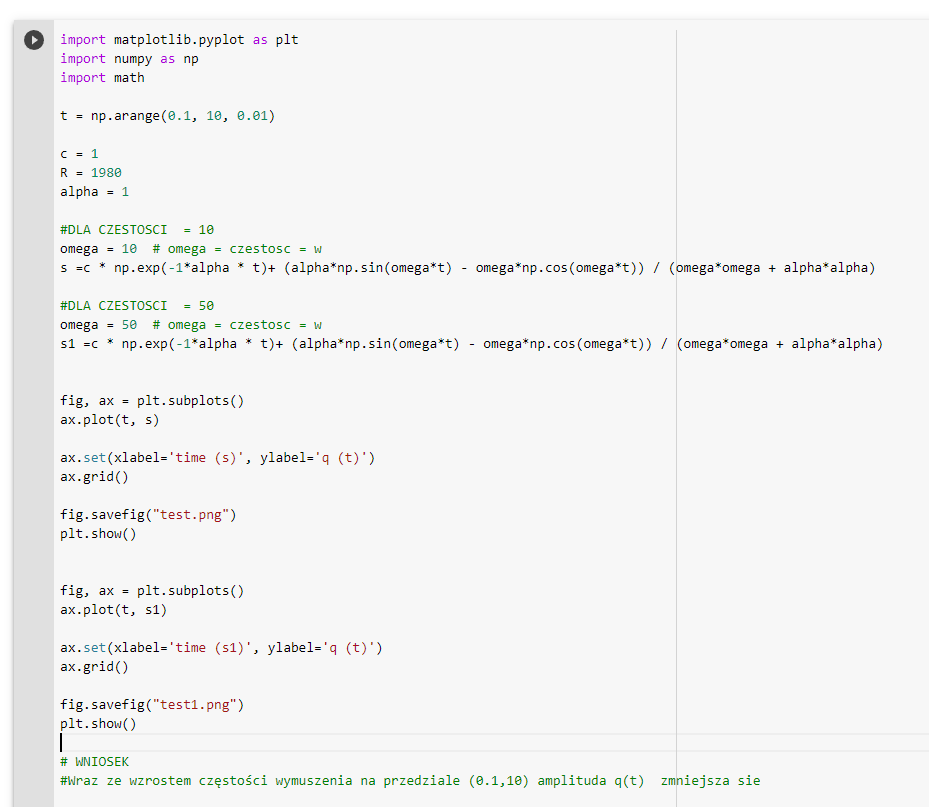
\includegraphics[scale=0.6]{./images/002.PNG} 
% \caption{\textit{Python code}.\newline }
% %do spisy tresci wersja skrócona
% \label{rys:logoup}
% \end{center}
% \end{figure}

\chapter{Mroczek Adrian - Rozwiazanie B  }


\begin{figure}[h]
\begin{center} 
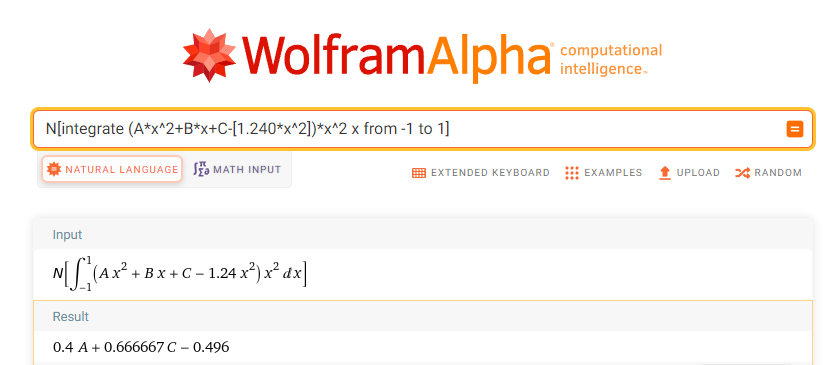
\includegraphics[scale=0.65]{./images/01a.PNG} 
\caption{\textit{Wyznaczanie równań do równania z trzema niewiadomymi cz1. }\newline }
%do spisy tresci wersja skrócona
\label{rys:logoup}
\end{center}
\end{figure}

\begin{figure}[h]
\begin{center} 
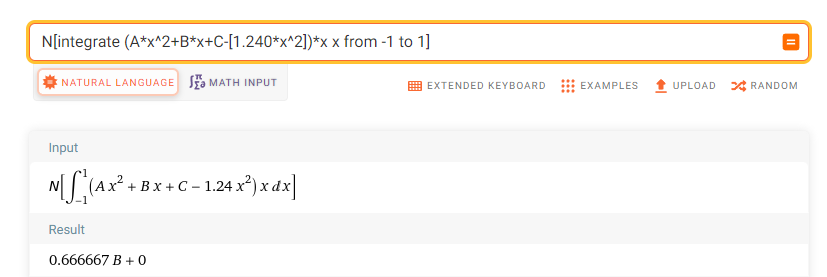
\includegraphics[scale=0.65]{./images/02a.PNG} 
\caption{\textit{Wyznaczanie równań do równania z trzema niewiadomymi cz2.}\newline }
%do spisy tresci wersja skrócona
\label{rys:logoup}
\end{center}
\end{figure}

\begin{figure}[h]
\begin{center} 
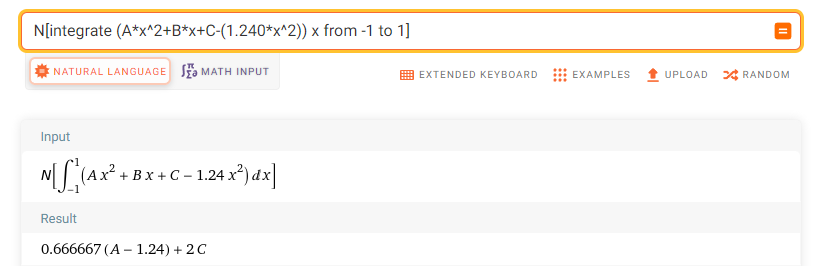
\includegraphics[scale=0.65]{./images/03a.PNG} 
\caption{\textit{Wyznaczanie równań do równania z trzema niewiadomymi cz3.}\newline }
%do spisy tresci wersja skrócona
\label{rys:logoup}
\end{center}
\end{figure}

\begin{figure}[h]
\begin{center} 
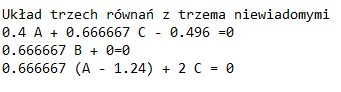
\includegraphics[scale=1.5]{./images/04a.PNG} 
\caption{\textit{Podsumowanie wyników powyższych obliczeń.}.\newline }
%do spisy tresci wersja skrócona
\label{rys:logoup}
\end{center}
\end{figure}

\begin{figure}[h]
\begin{center} 
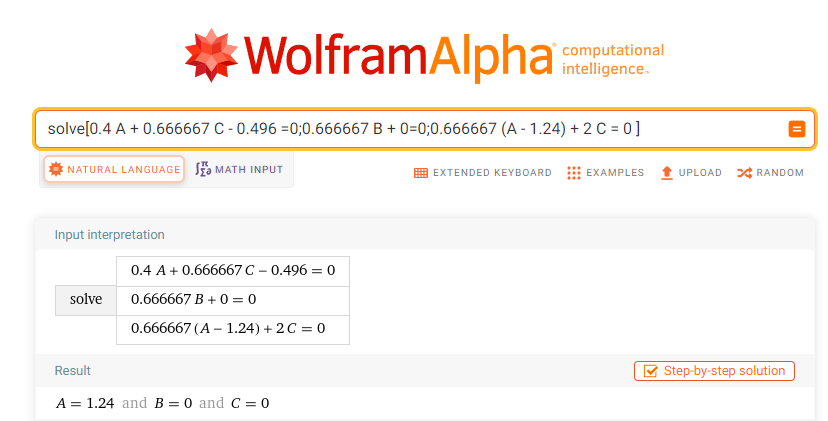
\includegraphics[scale=0.6]{./images/05a.PNG} 
\caption{\textit{Obliczenie wspólczynników A,B,C }.\newline }
%do spisy tresci wersja skrócona
\label{rys:logoup}
\end{center}
\end{figure}

\begin{figure}[h]
\begin{center} 
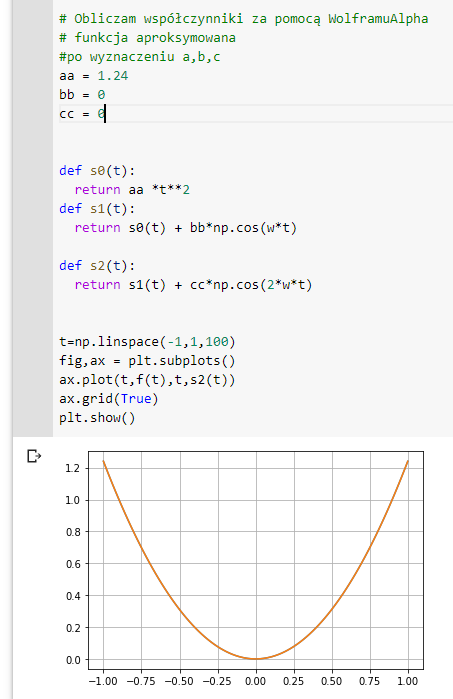
\includegraphics[scale=1.2]{./images/06a.PNG} 
\caption{\textit{Sprawdzenie dokładności znalezionego rozwiązania poprzeż narysowanie obu funkcji z użyciem języka Python. }\newline }
%do spisy tresci wersja skrócona
\label{rys:logoup}
\end{center}
\end{figure}


\chapter{Linki }

https://www.overleaf.com/read/qwpxdjkkkkqv \newline
https://github.com/mroczek-adrian/MroczekAdrianPrzetwarzanieSygnalow \newline
https://www.wolframalpha.com/  \newline

\end{document}